\subsection{Rayos x: Funciones de distribución de pares}

\begin{figure}[h!]
    \centering
    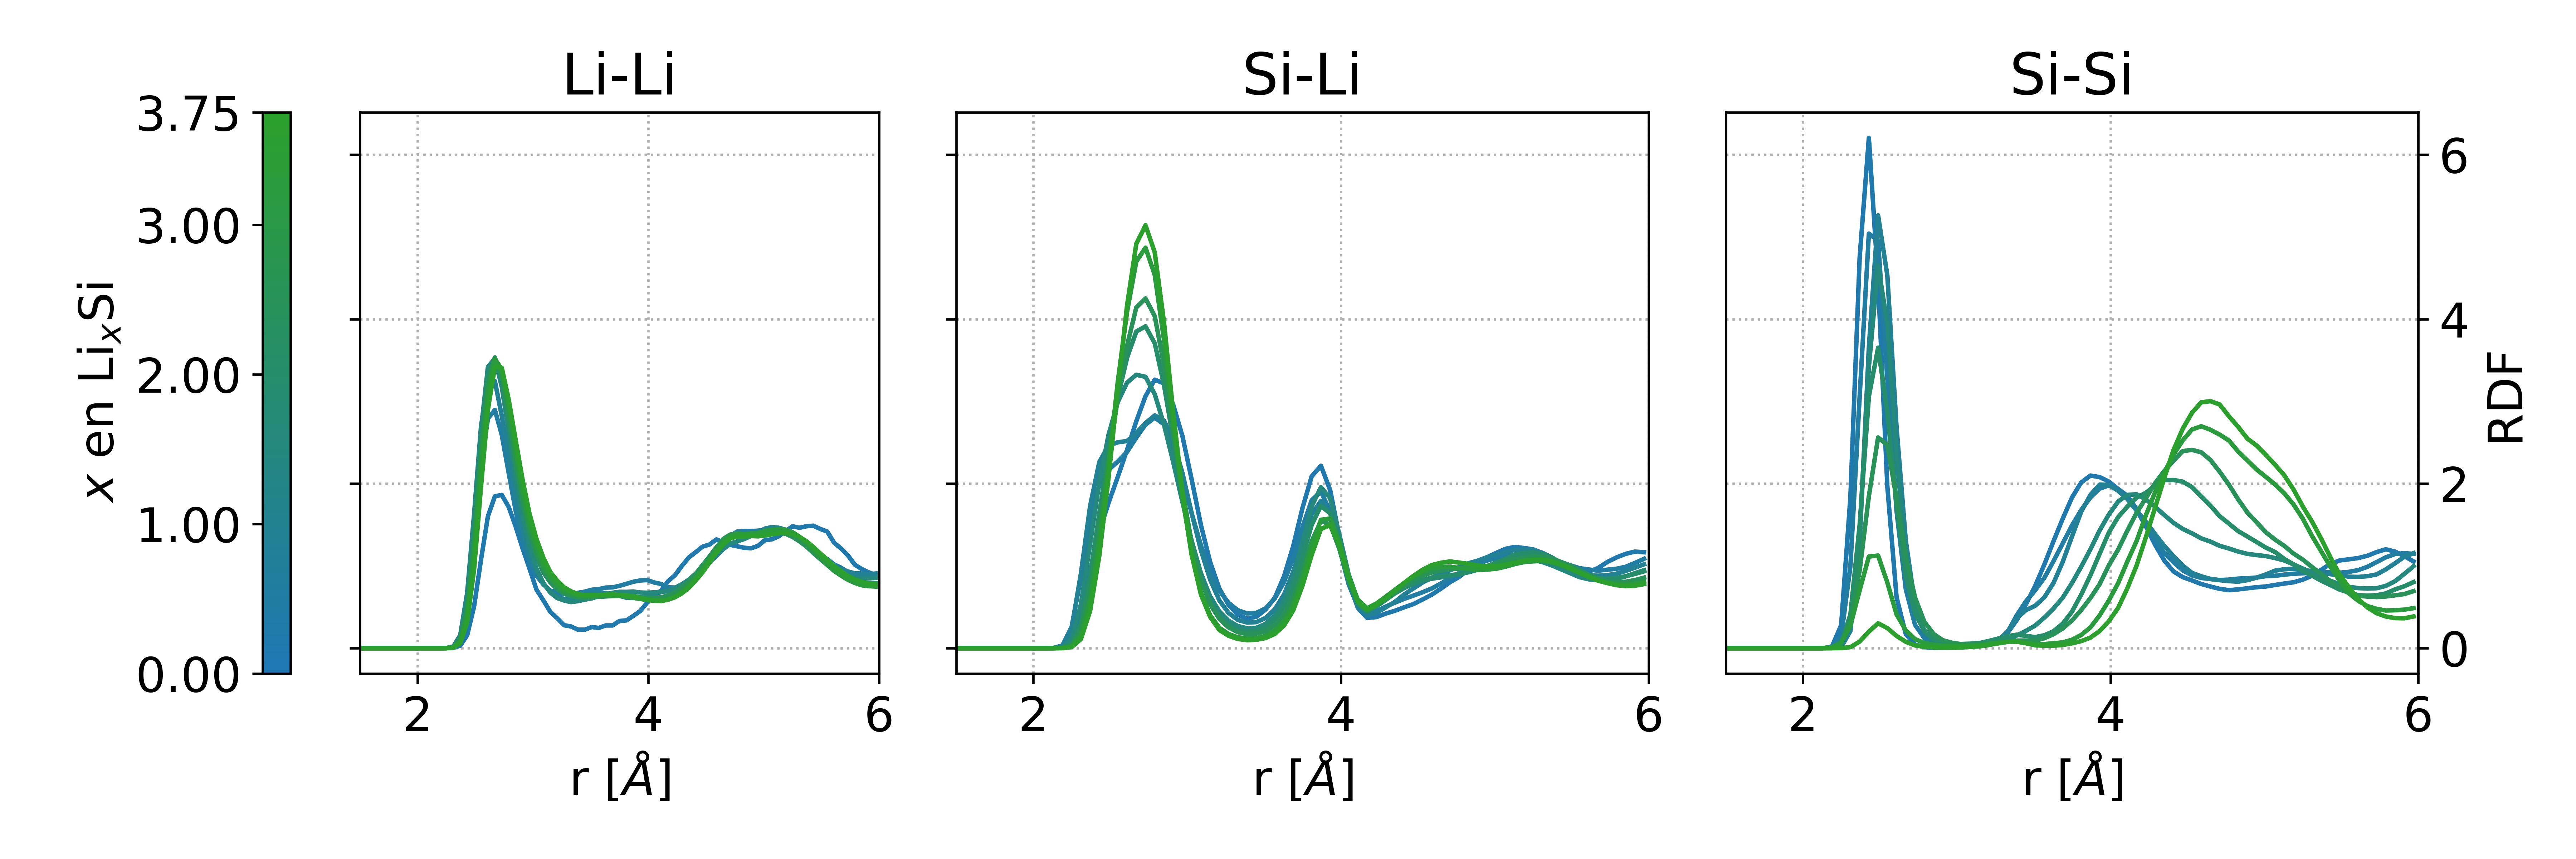
\includegraphics[width=\textwidth]{Silicio/prediccion/resultados/xray/prdfs.png}
    \caption{RDFs parciales para Li-Li, Si-Li y Si-Si para los valores $x$ en 
    Li$_x$Si optimizados. El color de la curva cambia de azul (predominio del Si)
    a verde (predominio del Li). Las barras de error son menores que el ancho de 
    las líneas.}
    \label{fig:prdfs}
\end{figure}

\begin{figure}[h!]
    \centering
    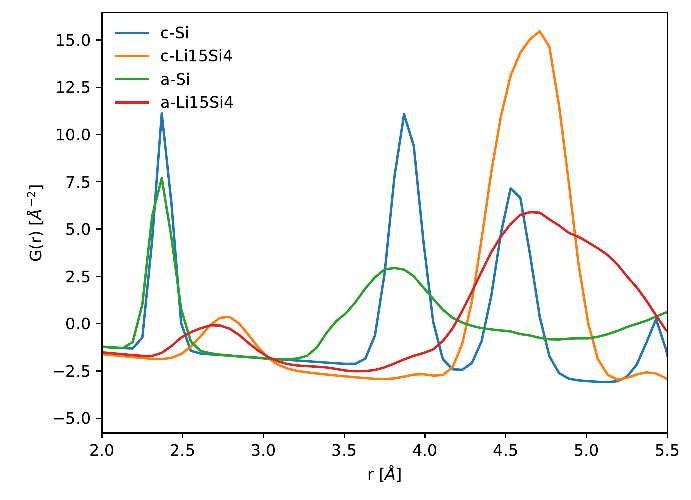
\includegraphics[width=.7\textwidth]{Silicio/prediccion/resultados/xray/gofrs.png}
    \caption{Funciones de distribución de pares $G(r)$ de estructuras 
    cristalinas y amorfas utilizadas para calcular las curvas de la Figura 
    \ref{fig:pdfs}.}
    \label{fig:gofrs}
\end{figure}

\begin{figure}[h!]
    \centering
    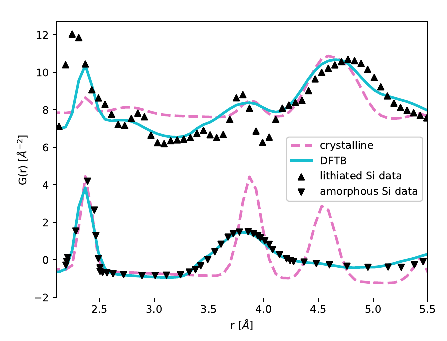
\includegraphics[width=.7\textwidth]{Silicio/prediccion/resultados/xray/pdfs.png}
    \caption{Funciones de distribución de pares $G(r)$ para Si amorfo y 
    completamente litiado contrastadas con datos experimentales. Los triángulos 
    que apuntan hacia abajo corresponden al experimento de a-Si de Laaziri, 
    mientras que los que apuntan hacia arriba corresponden al experimento de 
    Key \textit{et al.}. Las curvas DFTB azules consideran tanto las estructuras 
    cristalinas y amorfas. Las contribuciones de cada una están en la Tabla 
    \ref{t:w-gofrs}. Los datos de datos del Si litiado tienen una contribución 
    extra de 8 \AA$^{-2}$ para tener las dos curvas en el mismo gráfico. 
    Las barras de error son menores que el ancho de las líneas.}
    \label{fig:pdfs}
\end{figure}
